% Candidate prior networks used by the combustion experiment suite.
% orx TikZ layout guidance; the user requested the manuscript's LaTeX fonts.
\documentclass[10pt]{article}
\usepackage[T1]{fontenc}
\usepackage[utf8]{inputenc}
\usepackage[paperwidth=4.8in,paperheight=2.65in,margin=0pt]{geometry}
\usepackage{amsmath,tikz}
\usetikzlibrary{arrows.meta,positioning,calc}
\definecolor{coreblue}{HTML}{0072B2}
\pagestyle{empty}
\setlength\parindent{0pt}
\tikzset{
  orx/.style={font=\fontsize{9}{11}\selectfont,
    >={Stealth[round,length=4.5pt,width=3.5pt]},line width=.6pt},
  observable/.style={circle,draw=black!65,fill=white,minimum size=7mm,inner sep=0pt},
  explanatory/.style={observable,dashed,draw=coreblue,fill=coreblue!5},
  flow/.style={->,draw=black!65},
  description/.style={font=\fontsize{8.5}{10}\selectfont,text=black!85},
}
\begin{document}
\begin{minipage}[c][2.65in][c]{4.8in}
\centering
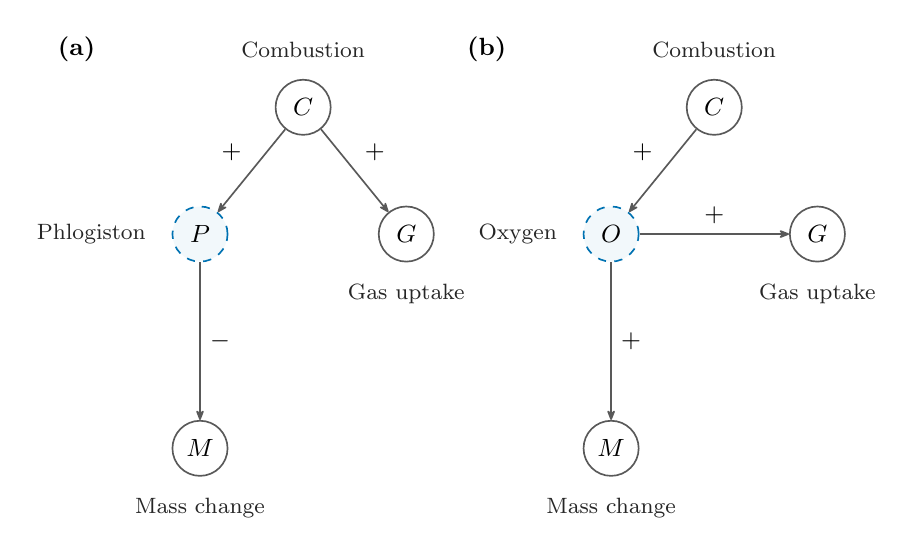
\begin{tikzpicture}[orx]
  \node[observable] (c) {$C$};
  \node[description,above=1.5mm of c] (ctitle) {Combustion};
  \node[left=16mm of ctitle] {\textbf{(a)}};
  \node[explanatory,below left=11mm and 8mm of c] (p) {$P$};
  \node[observable,below right=11mm and 8mm of c] (g) {$G$};
  \node[observable,below=20mm of p] (m) {$M$};
  \node[description,left=2mm of p] {Phlogiston};
  \node[description,below=1.5mm of g] {Gas uptake};
  \node[description,below=1.5mm of m] {Mass change};
  \draw[flow] (c) -- node[above left,font=\small] {$+$} (p);
  \draw[flow] (c) -- node[above right,font=\small] {$+$} (g);
  \draw[flow] (p) -- node[right,font=\small] {$-$} (m);

  \node[observable,right=45mm of c] (co) {$C$};
  \node[description,above=1.5mm of co] (cotitle) {Combustion};
  \node[left=16mm of cotitle] {\textbf{(b)}};
  \node[explanatory,below left=11mm and 8mm of co] (o) {$O$};
  \node[observable,below right=11mm and 8mm of co] (go) {$G$};
  \node[observable,below=20mm of o] (mo) {$M$};
  \node[description,left=2mm of o] {Oxygen};
  \node[description,below=1.5mm of go] {Gas uptake};
  \node[description,below=1.5mm of mo] {Mass change};
  \draw[flow] (co) -- node[above left,font=\small] {$+$} (o);
  \draw[flow] (o) -- node[above,font=\small] {$+$} (go);
  \draw[flow] (o) -- node[right,font=\small] {$+$} (mo);
\end{tikzpicture}
\end{minipage}
\end{document}
